\section{Подготовка к проведению эксперимента}

Для программной реализации системы оценки производительности
алгоритмов оптимизации, необходимо спланировать эксперимент,
разработать систему для проведения эксперимента, выбрать инструменты для ее реализации.

\subsection{Планирование эксперимента}

Цель эксперимента — выявить преимущества и недостатки тех или иных видов
оптимизации гиперпараметров и их влияния на время обучения и производительность
модели.

Входные данные — набор текстов писем электронной почты, для каждого из которых
заранее известно, является это письмо спамом или нет.

Выходные данные — оценка нескольких обученных на входных данных классификаторов спама.

Для удобства проведения эксперимента ограничимся алгоритмами роевого интеллекта,
которые работают по общему принципу, а метод роя частиц уже показал хорошие
результаты в этой области \cite{IEEE}.

План проведения эксперимента:

\begin{itemize}
      \item[—] Подготовить данные для эксперимента;
      \item[—] Предварительно обработать данные. Разделить данные на тренировочный
            и тестовый наборы;
      \item[—] Настроить параметры алгоритма машинного обучения;
      \item[—] Реализовать алгоритм глобальной оптимизации функции на основе того или иного природного алгоритма;
      \item[—] Реализовать объектную функциию, подлежащую оптимизации алгоритмом роевого интеллекта.
            Эта функция должна вычислять оценку модели МО для каждой частицы с новыми параметрами, а
            возвращать среднее арифметическое от вектора этих параметров.
            Оценочной функцией может служить как одна из \ref{Scorer}, так и
            нестандартная весовая функция;
      \item[—] Обучить модель с использованием полученных гиперпараметров;
      \item[—] Протестировать модель на тестовом наборе данных;
      \item[—] Оценить производительность модели, вычислив величины из \ref{Scorer} на
            тестовом наборе;
      \item[—] Повторить экспепримент, получив те же параметры с использованием
            других подходов к оптимизации, описанных в \ref{optimization};
      \item[—] Повторить эксперимент для другого природного алгоритма;
      \item[—] Провести сравнительный анализ получившихся оценок с целью выявления
            преимуществ и недостатков тех или иных видов оптимизации и их влияния на
            время обучения и производительность модели;
      \item[—] Объяснить полученные результаты эксперимента, сделать соответствующие выводы;
      \item[—] Обозначить направление дальнейших исследований.
\end{itemize}

\subsection{Архитектура системы для проведения эксперимента}

Механизм обнаружения спама должен иметь возможность работать с электронной почтой,
включающей html-заголовки и другую лишнюю в контексте данной задачи информацию.
В связи с этим набор входных данных подлежит предварительной обработке.

Данные также подлежат разделению на тренировочный и тестовый наборы.

Задаются начальные параметры алгоритма, желаемое значение оценочной функции (например, $Accuracy$),
число частиц, максимальное количество итераций. Затем на тренировочном наборе данных
проводится обучение модели с перекрестной проверкой на различных наборах
гиперпараметров, предоставляемых оптимизационным алгоритмом. Процесс продолжается
до тех пор, пока не будет достигнуто желаемое значение оценки алгоритма или
максимальное число итераций.

Затем модель, обученная на лучших параметрах, тестируется на тестовом наборе данных,
осуществляется оценка производительности полученной модели.

Рисунок \ref{scheme} представляет процесс реализации описанной системы.

\begin{figure}[H]
      \centering
      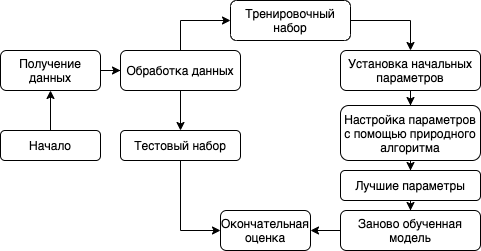
\includegraphics[width=140mm]{static/prog.png}
      \caption{Схема процесса обучения модели}
      \label{scheme}
\end{figure}

\subsection{Выбор инструментов для реализации системы}

Для реализации системы выбран язык программирования Python версии 3.9 или выше,
поскольку его использование обеспечивает наличие множества библиотек,
предназначенных для машинного обучения.

Реализации описанных в \ref{ML} алгоритмов машинного обучения
можно найти в библиотеке Scikit-Learn. Scikit-Learn —
библиотека машинного обучения, написанная на Python, довольно популярная
среди ученых-вычислителей. Она может похвастаться простым в использовании
интерфейсом и содержит множество инструментов для машинного обучения, в том числе
для классификация, предварительной обработки, кластеризации и регрессии данных.
Многие из этих алгоритмов могут быть полезны "из коробки", но чтобы получить
лучшую производительность, гиперпараметры должны быть настроены под конкретную
проблемную область, в которой алгоритм будет использоваться. Для такой настройки
будут использоваться алгоритмы роевого интеллекта, такие как, например, Firefly, Ant
Colony Optimization и Bee Colony Optimization.
